\documentclass[conference]{IEEEtran}

\usepackage{cite}
\usepackage{amsmath,amssymb}
\usepackage{booktabs}
\usepackage{graphicx}
\usepackage{microtype}
\usepackage[hidelinks]{hyperref}
\usepackage{xcolor}

% IEEE centers a page containing only a double-column float by default.  The
% manuscript includes a deliberately tall structural-comparison figure, so keep
% such a page top-aligned for normal conference-paper reading order.
\makeatletter
\setlength{\@dblfptop}{0pt}
\setlength{\@dblfpsep}{8pt}
\setlength{\@dblfpbot}{0pt plus 1fil}
\makeatother

\begin{document}

\title{StructIRES: Structure-Aware IRES Recognition and\
Constraint-Guided Optimization of Full-Length IRES Sequences}

% Replace this anonymous block only after confirming BIBE's review policy and
% authorship/affiliation order with the supervisor.
\author{\IEEEauthorblockN{Anonymous Authors}
\IEEEauthorblockA{Anonymous Institution\\
China\\
Contact information withheld for review}}

\maketitle

\begin{abstract}
Sequence-score optimization can select full-length internal ribosome entry site
(IRES) variants that drift from the parent thermodynamic ensemble, while
reporter-trained recognition scores do not necessarily transfer to direct-RNA
measurements. We introduce \textsc{StructIRES}, a two-stage framework. Its
completed \textsc{StructIRES-Rank} component is a generator-agnostic,
assay-aware rank-selection layer that combines a released IRES language-model
ensemble with parent-relative energy, global pairing-profile, and
high-confidence ensemble-anchor constraints; its structure-aware recognition
component is specified for a separate validation-locked evaluation. In a
controlled experiment over
ten experimentally supported full-length IRES seeds and three frozen mutation
pools, every method selects 50 variants from the same 512 candidates. Compared
with score-only selection, \textsc{StructIRES-Rank} reduces absolute minimum
free-energy deviation from 4.021 to 0.666 kcal/mol, pairing-profile distance
from 0.164 to 0.037, and increases parent-anchor retention from 0.646 to
0.955. It also improves an independent held-out direct-RNA computational proxy
from 0.419 to 0.435 (paired gain 0.0158; 95\% bootstrap interval
0.0079--0.0242). A public IAPV direct-RNA mutational scan further supplies an
assay-derived edit-risk guardrail. The results establish computational
candidate enrichment and structural preservation, rather than experimentally
verified translation improvement. Recognition results not yet produced by the
locked protocol are explicitly reported as pending rather than inferred from
design outcomes.
\end{abstract}

\begin{IEEEkeywords}
RNA design, internal ribosome entry site, RNA secondary structure, constrained
optimization, translation regulation
\end{IEEEkeywords}

\section{Introduction}

Internal ribosome entry sites (IRESes) enable cap-independent translation and
are useful regulatory components in RNA engineering. Their function is not
defined by a short motif alone: sequence context, alternative RNA structures,
host factors, cargo, and assay architecture can alter the measured output.
Consequently, a design procedure that only maximizes an IRES-recognition score
can produce candidates whose apparent improvement is disconnected from the
structural state of an experimentally supported parent.

Recent deep-learning work established IRES identification and evolutionary
sequence optimization baselines using 46,774 labelled sequences
\cite{chu2026iresai}. The dominant source, however, is a 174-nt
DNA/lentiviral reporter library \cite{weingarten2016ires}; it is not identical
to full-length or direct-RNA settings. We reproduced the released RNA-FM and
UTR-LM classifier summaries on their native repeated holdouts
(AUROC/AUPR/F1: $0.778/0.614/0.510$ and $0.765/0.581/0.493$,
respectively), but an all-checkpoint RNA-FM ensemble reached only AUROC 0.600
on a zero-shot direct-RNA evaluation. This motivates treating a historical
recognition model as a proposal signal rather than a complete activity oracle.

We present \textsc{StructIRES}, a two-stage framework linking structure-aware
IRES recognition with constrained full-length IRES optimization. Its
\textsc{StructIRES-Classifier} is a validation-clean RNA-FM re-training with
an MFE-contact encoder and gated residual; \textsc{StructIRES-Rank} is the
full-length constraint-guided selection component. The framework makes four
contributions:
\begin{enumerate}
  \item It tests whether an RNA foundation-model sequence prior is improved by
  contextual MFE base-pair features under matched validation-clean native
  folds, while reporting a separate identity-aware robustness audit.
  \item It combines sequence plausibility with parent-relative energy,
  thermodynamic ensemble, and ensemble-anchor preservation during design.
  \item It evaluates design alternatives on identical frozen candidate pools and
  selection budgets, isolating the value of each constraint.
  \item It uses direct-RNA evidence only as an explicitly assay-qualified
  evaluator or a parent-specific mutational guardrail, never as an inferred
  activity label for newly generated candidates.
\end{enumerate}

\begin{figure*}[t]
  \centering
  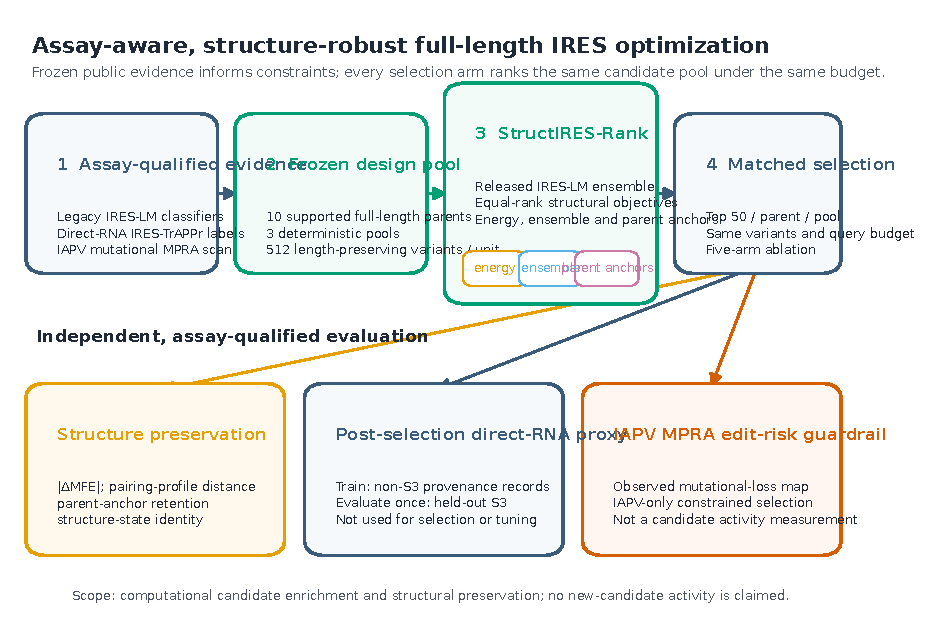
\includegraphics[width=0.96\textwidth]{figures/fig1_overview.pdf}
  \caption{Overview of \textsc{StructIRES}. \textbf{A}, the recognition
  component augments an author-style RNA-FM classifier with contextual
  residue-pair features over label-free ViennaRNA MFE contacts, fused through
  a zero-initialized gated residual. \textbf{B}, the completed design study
  ranks a shared, length-preserving mutation pool using a frozen released
  IRES-LM proposal score plus parent-relative energy, ensemble-profile and
  anchor-preservation objectives. \textbf{C}, direct-RNA resources are kept
  outside selection: they serve only as a held-out computational proxy or an
  IAPV-specific MPRA edit-risk guardrail.}
  \label{fig:overview}
\end{figure*}

\section{Method}

\subsection{Assay-aware evidence separation}
We retain source study, assay context, construct, cell type, sequence length,
and evidence level for every public record. Legacy DNA/lentiviral reporter
labels, circRNA-plasmid measurements, and direct-RNA measurements are not
pooled into one target. The released RNA-FM and UTR-LM classifiers form
IRES-LM, defined as the arithmetic mean probability over all ten released
checkpoints of each backbone. Direct-RNA labels are not used for checkpoint
selection, pool construction, ranking, or hyperparameter selection.

\subsection{Matched seeded optimization}
We start with ten experimentally supported full-length viral IRES parents.
For each parent, three deterministic mutation pools (seeds 42, 43, and 44)
contain 512 unique length-preserving substitution variants, each with at most
3\% edited positions. Every selection arm retains 50 candidates from the
same parent-specific pool. This fixes initial population, proposal set, edit
limit, and scorer-query budget across alternatives.

For a variant $x$ and parent $p$, lower is preferred for absolute MFE deviation
$|\Delta \mathrm{MFE}(x,p)|$ and global base-pairing-probability-profile
distance $D_{\mathrm{BPP}}(x,p)$. We also maximize weighted retention
$R_{\mathrm{anchor}}(x,p)$ of parent base pairs having ViennaRNA ensemble
probability at least 0.5 \cite{lorenz2011viennarna}. These are predicted
thermodynamic features, not experimentally mapped IRES motifs. The combined
method ranks the IRES-LM score and each structural quantity equally:
\begin{equation}
\operatorname{Rank}_{\mathrm{StructIRES}}(x)=
\frac{1}{4}\left[r_s(x)+r_e(x)+r_b(x)+r_a(x)\right],
\end{equation}
where $r_s$, $r_e$, $r_b$, and $r_a$ are within-pool ranks of sequence score,
energy preservation, pairing-profile preservation, and anchor retention.

\subsection{Independent evaluation and IAPV guardrail}
For the primary ten-parent study, a three-seed character 3--6-mer logistic
ensemble is trained after removing all S3-provenance direct-RNA records and
evaluated once on 222 held-out S3 records. It is a post-selection computational
proxy, not a candidate activity assay. We report parent-by-run means over 30
paired units and bootstrap intervals for differences from score-only selection.

For a separate IAPV case study, public direct-RNA mutational-scan tiles
\cite{may2026irestrappr} define a per-position edit-risk map: the median
non-negative measured translation reduction among overlapping observed tiles.
Uncovered positions receive the median observed risk. Adding this term is an
IAPV-specific conservation guardrail; it does not measure any newly designed
candidate.

\section{Results}

\subsection{Matched constraints preserve complementary properties}
Score-only selection yields high IRES-LM scores but substantial parent drift
(Table~\ref{tab:ablation}). Energy, global-ensemble, and anchor terms each
improve their intended structural quantity. The combined
\textsc{StructIRES-Rank} preserves all three simultaneously: it reduces mean
absolute MFE deviation by 83.4\%, pairing-profile distance by 77.4\%, and
increases parent-anchor retention by 0.309 relative to score-only selection.
All arms operate on the same 512 candidates per parent and retain the same 50
candidates, so this pattern cannot be attributed to a larger search budget.

\begin{table*}[t]
\centering
\caption{Matched full-length IRES optimization ablation. Values are mean $\pm$
sample SD across 30 paired parent-by-pool units (ten parents and three frozen
pools). Every arm retains 50 variants from the same 512 candidates. The
direct-RNA proxy is held out from selection and is computational only.}
\label{tab:ablation}
\resizebox{\textwidth}{!}{%
\begin{tabular}{lccccc}
\toprule
Selection method & $|\Delta$MFE| & Pairing $L_1$ & State identity & Anchor retention & Direct-RNA proxy \\
\midrule
IRES-LM score-only & $4.021\pm1.254$ & $0.164\pm0.027$ & $0.798\pm0.048$ & $0.646\pm0.075$ & $0.419$ \\
+ energy rank & $0.647\pm0.196$ & $0.118\pm0.024$ & $0.857\pm0.042$ & $0.766\pm0.062$ & $0.427$ \\
+ ensemble rank & $2.089\pm0.666$ & $0.055\pm0.014$ & $0.932\pm0.054$ & $0.915\pm0.026$ & $0.431$ \\
+ anchor rank & $2.093\pm0.580$ & $0.062\pm0.015$ & $0.924\pm0.063$ & $0.920\pm0.028$ & $0.431$ \\
\textsc{StructIRES-Rank} & $0.666\pm0.226$ & $0.037\pm0.010$ & $0.954\pm0.049$ & $0.955\pm0.015$ & $0.435$ \\
\bottomrule
\end{tabular}}
\end{table*}

The independent held-out direct-RNA proxy increases from 0.419 for score-only
selection to 0.435 for the combined method. The paired difference is 0.0158
(95\% bootstrap interval 0.0079--0.0242); combined ranking also exceeds the
energy, ensemble, and anchor ablations by 0.0086, 0.0046, and 0.0045,
respectively. These results support complementary roles for the three
structural constraints, while remaining an in-silico enrichment result.

\begin{figure*}[t]
  \centering
  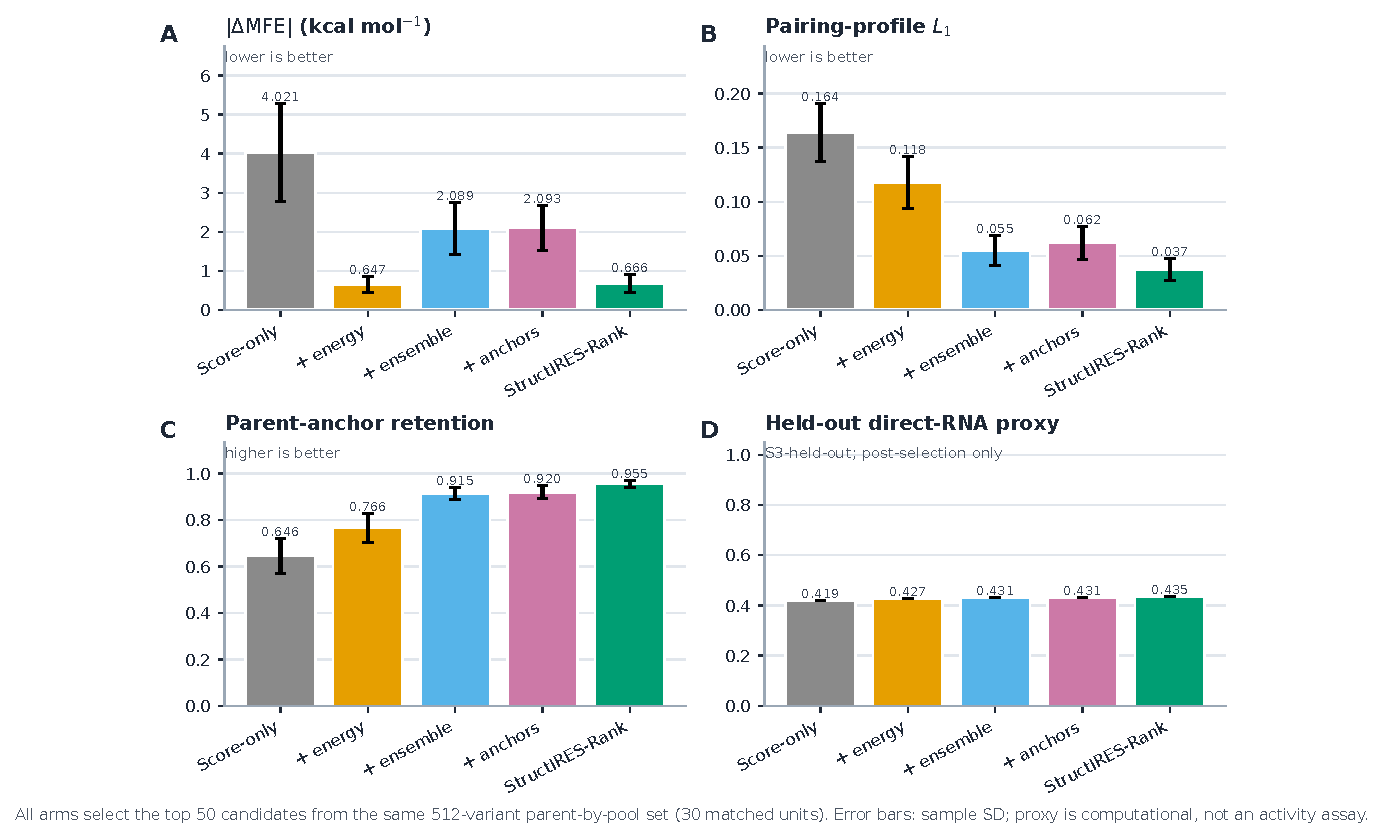
\includegraphics[width=0.98\textwidth]{figures/fig6_structires_ireslm_ablation.pdf}
  \caption{Matched \textsc{StructIRES-Rank} ablation. Each arm selects from
  the same candidate pool for every parent and random seed. Error bars are
  sample SD across 30 paired units. The direct-RNA proxy is held out from
  candidate selection and does not measure activity of selected variants.}
  \label{fig:ablation}
\end{figure*}

\subsection{Direct-RNA mutational knowledge acts as a transparent guardrail}
The public IAPV scan contains 208 A-substitution tiles covering 169 of 213
parent positions. For the IAPV-only matched ablation, adding its edit-risk term
decreases mean MPRA edit risk from $2.438\pm0.174$ to $1.782\pm0.087$
(paired difference $-0.656$, bootstrap interval $-0.933$ to $-0.480$). This
comes with a transparent MFE-preservation trade-off (0.641 to 0.887 kcal/mol),
so it is kept separate from the ten-parent headline result.

\begin{table}[t]
\centering
\caption{IAPV-only matched direct-RNA MPRA edit-risk guardrail. Both arms
select 50 variants from each of the same three 512-candidate pools. The risk
is induced by selected edits in observed parent mutational tiles; it is not a
new-candidate activity measurement.}
\label{tab:iapv}
\resizebox{\columnwidth}{!}{%
\begin{tabular}{lcccc}
\toprule
Method & Risk & $|\Delta$MFE| & Pairing $L_1$ & Anchors \\
\midrule
\textsc{StructIRES-Rank} & $2.438\pm0.174$ & $0.641\pm0.069$ & $0.032\pm0.006$ & $0.970\pm0.011$ \\
+ MPRA guardrail & $1.782\pm0.087$ & $0.887\pm0.131$ & $0.036\pm0.004$ & $0.963\pm0.008$ \\
\bottomrule
\end{tabular}}
\end{table}

\subsection{Assay shift motivates constrained rather than score-only design}
Released RNA-FM and UTR-LM checkpoint reruns recover their native benchmark
summaries, confirming that the published classifiers are meaningful baseline
proposal models. Yet on direct-RNA labels, RNA-FM checkpoint AUROCs range from
0.251 to 0.821 and the all-checkpoint ensemble has AUROC 0.600 and AUPR 0.058
at 5.1\% active prevalence. The released IRESfinder model is below random
ranking (AUROC 0.460) in the same transfer setting. Hence, the structural
terms are not presented as a substitute activity assay; they are conservative
constraints against over-optimizing an assay-specific score.

\section{Discussion}

\textsc{StructIRES} separates two related but distinct questions: whether a
sequence is IRES-like in a defined identification benchmark, and whether a
candidate can be optimized without losing the predicted structural state of an
experimentally supported parent. The completed \textsc{StructIRES-Rank}
component turns an IRES-recognition score into one component of a controlled
multi-objective selection procedure. Under a fixed proposal budget, it selects
candidates that retain parent energy and ensemble state more faithfully while
improving a held-out direct-RNA computational proxy. The IAPV case further
shows how direct-RNA mutational knowledge can be added transparently as a local
edit-risk guardrail.

The structure-aware recognition component is intentionally not claimed as a
completed performance gain in this draft. It becomes a contribution only if a
validation-locked run improves held-out ranking beyond the sequence baseline;
otherwise the paper remains a constrained-design study with transparent
sequence baselines.

The study has limitations. Secondary-structure predictions do not represent
all cellular or circular RNA effects, and the direct-RNA proxy is not a
functional assay. We therefore make no claim of experimentally verified IRES
activity for selected variants. Future work should evaluate the frozen
shortlists prospectively in matched direct-RNA settings and extend the
assay-aware framework to cargo and cell-context robustness.


\section*{Data and Code Availability}
The release package will contain frozen split and candidate-pool manifests,
executable baseline adapters, aggregate results, and scripts for all figures.
Large externally licensed assets and model weights will be referenced by
provenance manifests rather than redistributed. Candidate sequences remain
outside the public repository pending disclosure and publication review.

% The full IAPV secondary-structure case illustration is supplementary material:
% ../figures/fig7_iapv_secondary_structure.pdf

\section*{Acknowledgment}
To be completed after funding and authorship review.

\bibliographystyle{IEEEtran}
\bibliography{references}

\end{document}
